%!TEX root = ../template.tex
%%%%%%%%%%%%%%%%%%%%%%%%%%%%%%%%%%%%%%%%%%%%%%%%%%%%%%%%%%%%%%%%%%%
%% chapter1.tex
%% NOVA thesis document file
%%
%% Chapter with introduction
%%%%%%%%%%%%%%%%%%%%%%%%%%%%%%%%%%%%%%%%%%%%%%%%%%%%%%%%%%%%%%%%%%%

\typeout{NT FILE chapter1.tex}

\chapter{Introduction}
\label{sec:objectives}

\begin{itemize}
  \item Significance of non-verbal communication in social contexts

  \item Most common non-verbal cues studied in the literature are facial expressions and tone of voice, assuming a kind of social cue that can be observed as part of a conventional human-human exchange, when given attention. However, we can also take into account the changes that take place inside the body, that are not so well perceived without way of technological intervention.

  \item Affective Computing proposes the use of physiological activity to infer emotional states. However, these rely on linguistic descriptors

  achieving honourable breakthroughs in view of emotion recognition studies, constantly being pushed by the advancement of modern Machine Learning practices that are being used to interpret large-scale datasets.

  We recognise that these discrete representations become less meaningful when perceived in lack of contextual information.

  \item An emerging area of work considers the role of interactive systems for sharing of physiological activity  between it´s users holding a promising path for enhancing connectedness. However, the resulting artefacts tend to utilise raw forms of data representation, disregarding contextual information of the subject´s emotional state or surroundings.

  \item Aesthetics allow us to convey emotional meaning
  Aesthetics have been incorporated into a wide range of user-centred technologies, observed by the broader vision of third-wave Human-Computer Interaction. To which degree, novel systems have been capable of capturing and mediating the emotional experiences that manifest in our everyday life.
\end{itemize}

\section{Research Questions}
\label{sec:research_questions}

\begin{itemize}
%   \item How can we represent physiological activity in ways that are non-verbal?
%   \item How can aesthetics be incorporated into visuals, sound and haptic mechanisms to articulate and express emotional content?
%   \item What features can be extracted from each signal to gain information about the subject socio-affective state?
%   \item What specific social and emotional cues can be conveyed in a social context?
    \item Why should embodied sensor technologies be used to mediate speechless dialogue?
    \item What mediums are capable of producing emotionally meaningful representations of biosignals, suitable for social intervention?
    \item Adopting methods from modern Machine Learning and New Media practices, how can aesthetics be incorporated into visuals, sound and haptic mechanisms to articulate and express emotional content? And how do we encourage user empowerment and penalisation in Affective Systems?
\end{itemize}

Atypically from prevailing Affective Computing systems, the intention is not to infer or classify emotion, but rather create new opportunities for rich gestural exchange, unconfined to the verbal domain.

\section{Thesis Structure} % (fold)
\label{sec:structure}

\subsection{Chapter 1: Introduction}
The current section briefly sets out the underlying motivation and raises major research questions that run consistent throughout the thesis research.

\subsection{Chapter 2: Theoretical and Technical Concepts}

Chapter \ref{cha:technical_concepts} provides a background to the technical and theoretical concepts that form the foundation of thesis. To begin, we devide the proposed title into 4 constructs and establish the major themes of the research. This includes an overview of the different physiological signals commonly used in the field, along with fundamental concepts in Social Signal Processing and Somaestheitic design.

\subsection{Chapter 3: Literature Review}

In Chapter \ref{cha:lit_review}, we comment on some relevant literature covering the following key topics of interest: Affective Computing, Social Signal Processing, Machine Learning, Somaesthetic Design, biosignals in creative practice and sensor-based communication strategies.

\subsection{Chapter 4: Technical Contributions}

In Chapter \ref{cha:technical_contributions}, we will introduce and examine a set of hardware and software tools that were developed within the duration of the PhD and adopted for the purposes of augmenting nonverbal and collaborative interactions. This will range from specialized wearable devices for physiological data sensing to systems for processing and mapping this incoming data in meaningful ways.

\subsection{Chapter 5: Preliminary Actions}

Our Preliminary Actions \ref{cha:Preliminary_Actions} are initiated with an individualistic exploration of input-output mediums for physiological representation, forming a broad foundation of aesthetic affordances when testing with our own bodies. Transitioning from an introspective experience, we prepare engagements with a selection of specialist user-groups deemed suitable for providing new insights in a series of focus groups and participatory workshops.

\subsection{Chapter 6: Major Case Studies}

This will be followed by a series of use cases that were realised using the knowledge organised from the prior research actions. In Chapter \ref{cha:case_studies}. We will present a set of experimental systems developed during the PhD, each intended to establish a theoretical framework for designing systems for emotional exchange. Given this experimental methodology, a matured research space should provoke and sustain discussions around the socio-political implications of technological interventions and appropriation in preparation to be deployed in out-of-lab environments, eventually gearing towards pervasive engagement.

\subsection{Chapter 7: Results and Discussion}

Finally, we are able to reflect on a multi-layered research process and consolidate the overall outcomes that are rooted in the essential research appeal of the thesis. These are ultimately formulated as aesthetic considerations when designing for sensation, representation and communication in context of sensory intervention. In Chapter \ref{cha:conclusion} We open up to some the major limitations present in our work, disclosing the additional paths for investigation that remain unfulfilled, closing the thesis with a call for future work in the push towards aesthetic engagement with communication technologies.

\begin{figure}[htbp]
	\centering
	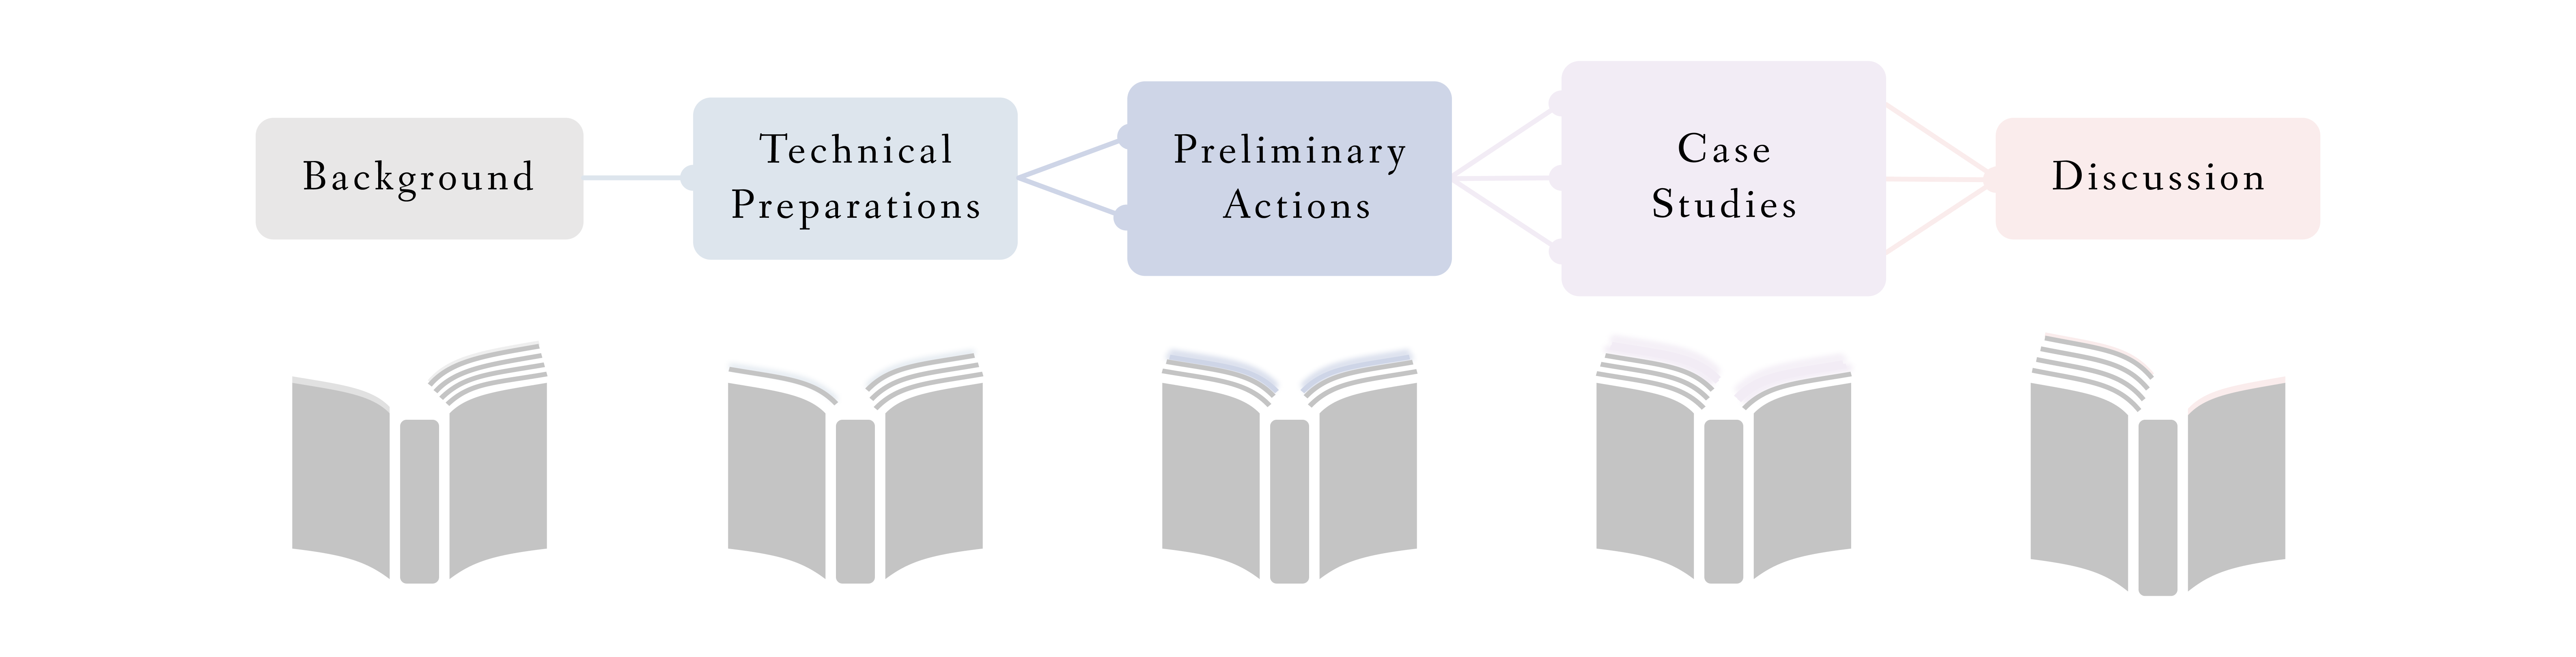
\includegraphics[width=1.0\textwidth]{Chapters/Figures/background/Sec1_Thesis_Structure}
	\caption{Thesis Structure Divided Into Five Stages}
	\label{fig:Concept_Venn}
\end{figure}

% \printbibliography[heading=subbibliography, segment=\therefsegment, title={\bibname\ for chapter~\thechapter}]
